%%%%%%%%%%%%%%%%%%%%%%%%%%%%%%%%%%%%%%
% This is the name of the style file.
%%%%%%%%%%%%%%%%%%%%%%%%%%%%%%%%%%%%%%
%
% phd  -> for a PhD dissertation
% ms   -> for an MS thesis
% If both phd and ms are used then phd will overide.  If none are used,
% then ms will be active by default.
%
% cpyr -> generate a copyright page
% lof  -> generate List of Figures
% lot  -> generate List of Tables
\documentclass[ms,cpyr,lof,lot]{uathesis}
%
%%%%%%%%%%%%%%%%%%%%%%%%%%%%%%%%
% List of any packages you use.
%%%%%%%%%%%%%%%%%%%%%%%%%%%%%%%%
%
\usepackage{amsmath}
\usepackage{amssymb}
\usepackage{epsfig}
\usepackage{graphicx}
\usepackage{changebar}
%
%%%%%%%%%%%%%%%%%%%%%%%%%%%%%%%%%%
% List of definitions you define.
%%%%%%%%%%%%%%%%%%%%%%%%%%%%%%%%%%
%
\def\ds{\displaystyle}
\def\E{\epsilon}
%

\title{Steve - A Programming Language for Packet Processing}
\author{Hoang Nguyen}
\conferraldate{May}{2016}

%The following commands specify the names and titles of people that
%will appear on the signature page.
%
%These four will always be needed.
\advisor{Andrew Sutton}
\chair{Timothy O'Neil}
\collegedean{John Green}
\gradschdean{Chand Midha}
%
%For a PhD dissertation, specify a coadvisor and three committee
%members, or four committee members only.  For an MS thesis use either
%one coadvisor or one faculty reader, not both.
%
%Typical commands for a PhD dissertation (uncomment only 4).
%\coadvisor{Name of Coadvisor}
\committee{Name of 1st Comm Member}
\committee{Name of 2nd Comm Member}
\committee{Name of 3rd Comm Member}
\committee{Name of 4th Comm Member}
%
%Typical commands for an MS thesis (uncomment only 1).
%\coadvisor{Andrew Sutton}
\facreader{NAME 1}
\facreader{NAME 2}

\begin{document}

\maketitle
\chapter{INTRODUCTION} \label{ch:intro}

The wave equation can be used to describe many physical phenomena.
Challenging topics in meteorology, acoustics, electro-magnetics, and
others involve solving the time-dependent wave equation.  Many of
these problems are described in an unbounded domain (i.e. there is no
boundary to reflect the outward traveling waves).  When an exact,
theoretical solution is unavailable, the lack of a boundary
prescription of accurate radiation conditions creates a problem for
numerical solutions.  The difficulty lies in is finding a way to do
calculations on an infinite domain using a computer with finite memory
in a finite amount of time and within a finite region.

\chapter{THE TWO DIMENSIONAL WAVE EQUATION} \label{2DWaveEquation}

Here is an example of a 'section' and a few equations.

\section{Recurrence Relation}

A series solution for the two-dimensional wave equation
\begin{equation}
\frac{1}{c^{2}}\frac{\partial^{2}u}{\partial t^{2}} = \frac{\partial^{2}u}{\partial r^{2}} + %
        \frac{1}{r}\frac{\partial u}{\partial r} + \frac{1}{r^{2}}\frac{\partial^{2}u}%
        {\partial\theta^{2}}                                                                 \label{waveEq}
\end{equation}
for outgoing waves is
\begin{equation}
u = \sum_{n=0}^{\infty}a_{n}(\theta)f^{n}(r,t),                                              \label{Soln}
\end{equation}
where
\begin{equation}
f^{n} = \sum_{k=0}^{\infty}r^{-k-\frac{1}{2}}f_{k}^{n}(ct-r).                                \label{function}
\end{equation} %look up reference.

You can reference a labeled equation by using the \textit{ref}
command.  For example, you can show that equations (\ref{Soln}) and
(\ref{function}) are a solution to equation (\ref{waveEq}).  (see the
file chap2.tex for the commands).

\section{Second Section Long Subtitle Second Section Long Subtitle Second Section Long Subtitle}
The text for the second section.  The text for the second section.
The text for the second section.  The text for the second section.
The text for the second section.  The text for the second section.
The text for the second section.  The text for the second section.

\subsection{First Subsection}
The text for the first subsection of the second section.  The text for
the first subsection of the second section.  The text for the first
subsection of the second section.  The text for the first subsection
of the second section.  The text for the first subsection of the
second section.  The text for the first subsection of the second
section.  The text for the first subsection of the second section.
The text for the first subsection of the second section.

\section{Third Section}
The text for the third section.  The text for the third section.  The
text for the third section.  The text for the third section.  The text
for the third section.  The text for the third section.  The text for
the third section.  The text for the third section.

\chapter{THE PACKET PIPELINE PROCESSING MODEL} \label{pipeline_model}

A packet comes into a data plane via an ingress port. This packet must go through a series of processing stages where it is analysed, modified, and ultimately forwarded out through an egress port. These processing steps are what is known as a \textbf{pipeline}.

The Steve programming language allows programmers to define their own pipeline applications. In the Steve processing model a pipeline is a composition of two types of processing stages: decoding stages and table matching stages. Each stage performs a set of operations on a packet, known as actions, and decides where to move the packet next based on certain conditions that the packet meets. A packet can be moved to another processing stage or it can be sent out of the pipeline.

The pipeline is thus a state machine. Each processing stage denotes a state in the machine. Each state has a set of conditions which, when met, causes the packet to transition states. This can be represented as a graph where each processing stage is a node on the graph and each state transition is an edge connecting stages. This is a valuable property as it allows the Steve programming language to analyse these pipelines and enforce certain logical, safety, and correctness guarantees about a user-defined pipeline.

Steve pipelines follow a run-to-complete model of execution. Once a packet enters the pipeline, each processing stage is consecutively applied to the packet until the programmer decides to forward or drop the packet.

\section{Decoding Stage} \label{decoder_desc}

When a packet is received on its ingress port, it is a chunk of raw, uninterpreted data. Before a packet can be processed and routed, its headers and fields must be decoded and extracted so that meaningful decisions can be made about what to do with the packet. The decoding stage is responsible for ensuring this happens.

Steve allows for programmers to specify \textit{how} and \textit{which} fields are extracted from packet headers. In other paradigms, the \textit{entire} packet is decoded from start to finish; all headers and all fields are extracted, then all fields are saved. This is what is considered a \textbf{full decode}. After this full decode, the decision making process on the packet begins using those saved fields. However, this method is inherently inefficient. Only certain fields and headers within a packet are ever really needed during the forwarding process. To compound this, different devices may care about different subsets of fields within a given packet. Decoding all of these fields does not make sense when only a smaller subset is ever necessary.

Full decodes waste valuable processing time. Efficiency is important when dealing with networking equipment which has to processes between 10Gbps to 40Gbps. Decoding fields which are not needed is equivalent to wasting clock cycles on the CPU which translates to slower performance.

This inherent inefficiency is why Steve proposes the idea of a \textit{partial decode}. Unlike similar SDN-focused programming languages, Steve is designed to allow programmers to specify the extraction of only specific fields rather than an entire header. Though the specification may be verbose in some cases, it makes programmers think very carefully about which fields they need and which fields they do not.

Additionally, Steve proposes that not all headers need to be decoded. For example, if a networking application only needs to forward using MAC addresses, there is no reason to waste time extracting fields from IPv4 or IPv6 headers, and so on.

\subsection{Packet Context} \label{context_desc}

A stage often needs to use data created by prior stages. As a packet moves between stages, information such as the position and length of extracted fields and headers must be saved for recovery later in the pipeline. To save this information, Steve applications use a data structure called the packet \textbf{context}. Specifically, a Steve context saves the following data:

\begin{itemize}
\item The logical and physical port the packet arrived on.
\item The length of the packet frame.
\item A tunnel identifier.
\item The offset and length of a field in the packet.
\item The offset of a header in the packet.
\item An action set that can be written to.
\end{itemize}

Extracted fields and headers get saved in \textbf{binding environments} contained within the context. The term \textbf{environment} refers to a function that maps names (in this case field and header names) to their storage location during runtime \cite{compilers1}. The mapping of those storage locations to the values held there is known as \textbf{state}. There is a binding environment for fields and headers respectively.

Figure \ref{fg:ContextEnv} depicts the binding environment. The field binding environment is used to map fields to offset-length pairs where that field can be found in a packet. The packet header environment similarly maps headers to offsets where that header can be found in a packet. These mappings are known as \textit{bindings}.

Since any given packet can contain one or more of any field or header with the same name, the environments maintain a stack for every field and header. These stacks are what are called \textit{binding stacks}. By extension, this means an environment is actually a mapping of fields to binding stacks. When the value of a field is needed, the topmost binding on the binding stack shall be used to recover the state of that field.

The implementation of environments in Steve is a fixed-sized array where each element in the array is a fixed-sized binding stack. Each index in the array represents a unique field or header name extracted by the Steve application. The compiler is responsible for associating all unique fields extracted during the decoding stage to unique integer indices into the array. The same is done for all unique headers. This provides constant time lookup of field bindings without the overhead of hashing found in environments which use complex name mappings.

\begin{figure}
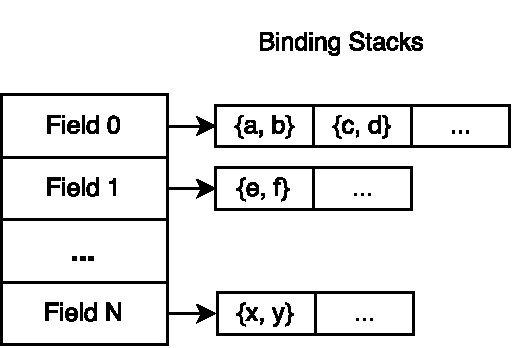
\includegraphics[scale=0.75,natwidth=203,natheight=298]{context}
\caption{The binding environment inside a context used to store the length and offset of fields, or the offset of headers. On the left, fields one through sixteen represent the fields that can be extracted. Each field maintains a binding list (stack). Each element in the binding list is a binding which stores the offset and length where each instance of that field can be found in the packet. }
\label{fg:ContextEnv}
\end{figure}

Figure \ref{fg:ContextEnvWorking} demonstrates how data is stored in the context as it is being decoded. The example is a packet which contains an encapsulated IPv4 header commonly used in IP tunneling. In the ethernet decoding stage which extract the \texttt{src}, \texttt{dst}, and \texttt{type} field are extracted and stored in the context. Next we determine that IPv4 follows based on the \texttt{type} field. We extract IPv4 \texttt{dst} and \texttt{protocol}. The \texttt{protocol} field tells us we have another IPv4 header after the current one. We move to decode that and once again we extract IPv4 \texttt{dst} and \texttt{protocol}. Note how the new values of IPv4 are pushed on top of the binding stack. Any further usage of those fields will use the latest values extracted for those fields. Keep in mind that this means any usage of the first set of IPv4 \texttt{dst} and \texttt{protocol} must occur before the decoding of the second IPv4 header.\

\begin{figure}
TODO: Make an image for this.
\caption{A context environment in action during runtime.}
\label{fg:ContextEnvWorking}
\end{figure}

The \textbf{action set} is the other major data structure contained within the context. The action set is a set of actions which have been written to the context for deferred execution using a \texttt{write action} (see Section \ref{action_tut}). Upon reaching a designated egress port, the action set is executed right before the packet is output.

\section{Table Stage} \label{table_desc}

Table stages handle matching against extracted fields, i.e. classification, and perform a sequence of desired actions on like-classified packets. This is done through a mechanism known as a flow table \cite{openflow_spec}.

A \textbf{flow table} is composed of a set of \textbf{flow entries}. A flow entry is composed of \textbf{match fields}, a \textbf{priority}, a set of \textbf{actions}, and miscellaneous additional data. Each table specifies a set of key fields that together make up a \textbf{key} for that table. For each key field, each flow entry has a corresponding value, known as a \textbf{match field}, such that every flow entry in the table is uniquely identified by its match fields and its \textbf{priority}.

When a packet reaches a table matching stage, the fields comprising the table's key are extracted from the context. Lookup into the table retrieves all flow entries whose match fields can correctly match the field values from the packet. The flow entry whose priority is highest is selected. The \textbf{actions} of the flow entry are executed on the packet.

If no such flow entry matches against the packet's field values, the \textbf{miss case} flow entry is applied to the packet instead. Flow entries can be user defined. By default, a miss in a table results in the packet being dropped. Miss cases always have the lowest possible priority amongst flow entries and each match field can be considered a wildcard.

The mechanic of table matching is not distinctly different from those of relational or SQL tables. In fact, Frenetic, another packet processing language, uses SQL-inspired syntax to classify flows \cite{frenetic_paper1}. If we make this comparison, a flow table is analogous to a SQL table, the concept of a key is the same for both, and a flow entry is analogous to a tuple in a SQL table. Each packet and its fields constitute the actual "query" into the table.

\section{Pipeline Composition} \label{pipeline_comp_desc}

Kinds of processing stages can be interleaved together in any order within the pipeline. This means that Steve is capable of supporting different packet processing paradigms found in other research such as POF and P4. With the Steve pipeline specification language a user can specify that a pipeline does:

\begin{enumerate}
\item \textbf{A full decode of the packet followed by a sequence of tables.} Packets coming to the pipeline have all necessary headers and fields are decoded and saved in the runtime context first. The packet is then dispatched to the first table in the pipeline. From there, matched flows within the tables dictate which table the packet is sent to next or which port the packet is forwarded to.
\item \textbf{A chain of partial decodes and table lookups.} Packets coming to the pipeline get partially decoded and dispatched to a table. The flow within that table could carry the packet to another table, another decoder, or forward it out of the network. The pipeline in this case in a chain of alternating sequences of decoding stages and table matching stages.
\item \textbf{Only decodes.} In some special cases, it may not even be necessary to go to a table matching stage. It may be possible to make a decision about the packet’s ultimate destination immediately upon evaluating a certain field within the packet using a simple conditional statement (if-statement, if-else statement, etc). Therefore, decoding stages also support the range of actions supported by flow entries, which can include outputting packets to a port or dropping it.
\end{enumerate}

Upon entering the pipeline, a packet must first go through at least one decoding stage before moving to the next processing stage. From there, the packet flows from one stage of the pipeline to the next. With each stage, certain conditions are evaluated which will determine where the packet must flow next. Finally, the packet will exit the pipeline either through a port(s) or by being dropped and discarded.

\chapter{Tutorial} \label{tutorial}

This chapter provides a tutorial on the syntax of Steve and using its language features. Steve's primary focus is to provide language features for declaring, specifying, and constructing the pipeline processing stages described in Chapter \ref{pipeline_model}. This chapter will explain how to represent packet headers, how to write decoding stages, how to write table stages, and how to use actions.

Throughout this chapter there be small semantic details mentioned when necessary. For complete details on the semantics of Steve, see the User's Guide in Chapter \ref{users_guide}.

For a complete reference of all Steve syntax, see Appendix \ref{ap:a}.

\section{Layouts} \label{layout_tut}

Before pipeline processing stages can be written, a \textbf{layout} is used to describe the physical structure of a packet header, i.e. what fields they have and the respective lengths of those fields. Figure \ref{fg:layout_syntax} provides the syntax for layout declarations in BNF notation.

A \textbf{layout declaration} is composed of a sequence of \textbf{field declarations}. Each field declaration corresponds to a field in a header. The type of each field declaration defines the length of the corresponding field in a header. Each field declaration in a layout must be written in the same order with which the field appears in a real instance of the header. If the ordering does not match, layouts will not function correctly during decoding stages. 

\begin{figure}
\begin{mdframed}
\begin{grammar}

<layout-decl> ::=
\textbf{layout} <layout-name> 
\textbf{\{}
	<field-decl> +
\textbf{\}}

<field-decl> ::=
<field-name> \textbf{:} <type> \textbf{;}

<type> ::=
<scalar-type>
\alt <layout-type>

<scalar-type> ::= <integer-type>

<integer-type> ::=
\textbf{int} [ \textbf{(} <integer-literal> \textbf{)} ]
\alt \textbf{uint} [ \textbf{(} <integer-literal> \textbf{)} ]

<layout-type> ::=
<layout-decl-id>

\end{grammar}
\end{mdframed}
\caption{Layout syntax for Steve in BNF.}
\label{fg:layout_syntax}
\end{figure}

A field declaration within a layout is limited to being one of two different types. The first of these types is scalar type (most often a signed/unsigned integer type). Integer types can be given with an optional bit-length precision, with the default being 32-bits if no precision is specified. This bit-length precision is used to determine the length of the field. An example of a layout corresponding to the ethernet header \cite{eth_std} can be seen in Figure \ref{fg:ethernet_layout_ex}. The \texttt{src} and \texttt{dst} fields are 48-bits, or 6 bytes, long. The \texttt{type} field is 16-bits, or 2 bytes, long.

\begin{figure}
\begin{lstlisting}
layout eth
{
  dst  : uint(48);
  src  : uint(48);
  type : uint(16);
}
\end{lstlisting}
\caption{An example of how the ethernet header is written in Steve.}
\label{fg:ethernet_layout_ex}
\end{figure}

The second supported type is layout type. This allows layouts to be nested together in case a programmer must deal with a header with structures nested inside them. In this case, a field declaration is used whose type is given as the identifier to layout declaration. Figure \ref{fg:nested_layout_ex} gives a trivial example of nested layouts.

\begin{figure}
\begin{lstlisting}
layout eth
{
  dst  : uint(48);
  src  : uint(48);
  vlan_tag : vlan;
  type : uint(16);
}

layout vlan
{
  tpid : uint(16);
  tci  : uint(16);
}
\end{lstlisting}
\caption{An example of a layout being nested inside another layout.}
\label{fg:nested_layout_ex}
\end{figure}

Keep in mind that a layout, though similar to a class, is not a class. Objects of layout type can never be created, they cannot contain member functions, and their fields must all be of scalar or layout type. Layouts are use to determine two things: what the offset of a given field is relative to the beginning of the header and the length of the field. These two pieces of information are important during decoding stages where these fields are extracted. In this way, layouts more closely translate to extraction rules used during the decoding process. 

The primary reason for this differentiation in Steve are dynamically-sized fields in packet headers. Headers potentially have fields whose memory size is predicated upon some value discovered during runtime. These fields are said to have \textbf{dynamically sized type}. Some examples of this are the \texttt{options} fields in IPv4, IPv6, and TCP headers. Consider that when objects of any type are constructed, stack space must be allocated for them. Except, it is impossible to stack allocate an object whose size is not known during compilation without some hint about its maximum size. Such objects can only be heap allocated, which Steve does not currently support. 

Furthermore, accessing these dynamically-sized fields, recovering their values, and performing operations on them would have to be done through special pointers to ensure the safety of such operations. For further details on layout limitations, refer to Section \ref{layout_guide} in the User's Guide.

Steve does not currently support dynamically sized types. This is a language feature that will eventually be added, but is outside the scope of this thesis. Because of this, fields whose lengths are dynamic cannot currently be declared, extracted, nor used. 

An IPv4 header example can be seen in Figure \ref{fg:ipv4_layout_ex}. Note that the \texttt{options} field is skipped due to the lack of dynamically sized types. Also note that Steve does not support non-byte aligned data types, and thus the precision of all integers are multiples of 8. Fields which are non-byte aligned must be merged to byte alignment and recovered using arithmetic operations (see Figure \ref{fg:assign_arith_ex} in Section \ref{decoder_tut} for an example). 

\begin{figure}
\begin{lstlisting}
layout ipv4
{
  version_ihl : uint(8);
  dscp_ecn    : uint(8);
  len         : uint(16);
  id          : uint(16);
  fragment    : uint(16);
  ttl         : uint(8);
  protocol    : uint(8);
  checksum    : uint(16);
  src         : uint(32);
  dst         : uint(32);
}
\end{lstlisting}
\caption{An example of how the IPv4 header is written in Steve. Note that the "options" field is not included because Steve does not currently support extraction or usage of dynamic length fields.}
\label{fg:ipv4_layout_ex}
\end{figure}


\section{Decoders} \label{decoder_tut}

\textbf{Decoders}, also referred to as decoding stages in the pipeline processing model,  are special purpose functions used to handle decoding and extracting fields in a given header. By chaining multiple decoders together, a user can construct a set of functions used to parse an entire packet. \textbf{Decoder declarations} are Steve's way of defining decoding stages. Figure \ref{fg:decoder_syntax} presents the syntax used to write decoders. Decoder declarations provide users the ability to:

\begin{itemize}
\item Declare which header is being decoded and which fields to extract from it.
\item Perform arithmetic and logical operations on fields.
\item Perform actions on the header. See Section \ref{action_tut} for examples of action usage.
\item Decide what processing stage comes next. Either the next header is determined and the packet is dispatched to that decoding stage, or the packet is dispatch to table matching.
\end{itemize}

\begin{figure}
\begin{mdframed}
\begin{grammar}

<decoder-decl> ::=
\textbf{decoder} <decoder-name> [\textbf{start}] 
\textbf{(} <layout-id> \textbf{)}
<block-statement>

<extract-decl> ::=
\textbf{extract} <field-name> \textbf{;}

<rebind-decl> ::=
\textbf{extract} <field-name> \textbf{as} <field-name-expr> \textbf{;}

<field-name> ::=
<layout-id> \textbf{.} <field-id>
\alt <field-name> \textbf{.} <field-id>

<field-access-expr> ::=
<layout-id> \textbf{.} <field-id>
\alt <field-access-expr> \textbf{.} <field-id>

\end{grammar}
\end{mdframed}
\caption{Decoder syntax for Steve in BNF.}
\label{fg:decoder_syntax}
\end{figure}

\subsection{Extractions} \label{decoder_extract_tut}

The primary goal of decoders is to extract fields from headers. Assume we wanted to write a decoder to extract the \texttt{src} and \texttt{dst} fields from an ethernet header. Remember, Steve allows for the partial decoding of packets, so if we do not need a field, in this case \texttt{type}, its not necessary to extract it. 

First, a layout for the ethernet header must be defined. In this case, the layout defined in Figure \ref{fg:ethernet_layout_ex} can be used. This layout will be used to determine the offset (location) and length of each field in the header during decoding. More details on this process can be found in Section \ref{decoder_guide}. 

After that, we can proceed to writing the decoder declaration. Figure \ref{fg:extract_ex} demonstrates how the extraction is written. We give this decoder declaration the name \texttt{eth\_decode} and specify the layout used to decode in the parenthesis following the name (in this case \texttt{eth}). A decoder can only extract fields from a header defined by this layout. If an attempt is made to extract a field from a different header a compiler error is emitted. The optional \texttt{start} keyword is attached to this decoder to denote that this decoder is the first stage in the pipeline. Ethernet is the most commonly used data link layer protocol, making it the most common header to start with. There can only be one starting decoder. 

To extract a field, the programmer writes an \textbf{extract declaration} which requires that a field be specified using a \textbf{field name}. A field name is used to refer to a field of a layout. For example \texttt{eth.dst} refers to the \texttt{dst} field of the \texttt{eth} layout.  Note that this is distinctly different from member access as the \texttt{eth} layout is not an object. 

The first extract declaration (\texttt{extract eth.dst;}) says that the decoder extracts the \texttt{dst} field of the \texttt{eth} header. The second extract declaration (\texttt{extract eth.src;}) says that the decoder extracts the \texttt{src} field of the \text{eth} header. 

\begin{figure}
\begin{lstlisting}
decoder start eth_decode(eth)
{
  extract eth.dst;
  extract eth.src;
  // More code to follow...
}
\end{lstlisting}
\caption{An example of how to extract \texttt{src} and \texttt{dst} fields from the ethernet header using a decoder. Note we do not extract the \texttt{type} field here.}
\label{fg:extract_ex}
\end{figure}

\subsection{Accessing Extracted Fields} \label{decoder_access_tut}

After extracting a field from a header, a programmer will almost certainly want to use the field in some kind of operation whether that be arithmetic or logical. To use the \textit{value} of an extracted field, a programmer uses a \textbf{field access expression}. Field access expressions have the same grammar as field names, but they can be used wherever any expression is valid. The behaviour of field access expressions is similar to how the name of a variable can be used to mean the value stored in that variable in C-like languages.

Figure \ref{fg:access_ex} demonstrates how the value of extracted fields can be used in Steve. In this scenario, we extract \texttt{eth.type} and use the value as a condition in a C-like if-else statement. We use this if-else statement to determine what the \texttt{type} field means. The IEEE ethernet standard says that if the \texttt{type} field is greater than or equal to hexadecimal \texttt{0x600}, then the value of the field is used to determine the kind of header encapsulated by the ethernet header \cite{eth_std}. Otherwise, if the \texttt{type} field is less than hexadecimal \texttt{0x05dc}, the field refers to the length of the ethernet frame.

\begin{figure}
\begin{lstlisting}
decoder start eth_decode(eth)
{
  extract eth.type;
  
  // Using a field access expression 
  // with logical operator >=
  if (eth.type >= 0x600)
  {
    // Then this is determines what
    // header comes next.
  }
  // Using a field access expression 
  // with logical operator <=
  else if (eth.type <= 0x05dc)
  {
    // Then this is the length field.
  }
  // ...
}
\end{lstlisting}
\caption{An example of accessing a field using the field access expression in an if-else statement.}
\label{fg:access_ex}
\end{figure}

Field access expressions can also be used in arithmetic operations, bitwise operations, and can be stored and assigned to local variables. Figure \ref{fg:assign_arith_ex} demonstrates how this can be done using an IPv4 decoder as an example. First it's shown that it's possible to assign the value of the header's \texttt{len} field to a local variable named \texttt{pktlen}. Next the example shows how to recover \texttt{ihl} and \texttt{version} from a single field (to deal with the limitation of only supporting byte-aligned fields). Note that it is possible to use bitwise and shift operations on fields as well. After that, the example demonstrates subtraction on the \texttt{ipv4.len} field to determine what the time-to-live will be after the packet leaves the current device.

\begin{figure}
\begin{lstlisting}
decoder ipv4_decode(ipv4)
{
  extract ipv4.len;
  extract ipv4.version_ihl;
  extract ipv4.ttl;
  
  // We can assign to variables
  var pktlen : uint = ipv4.len;
  
  // We can perform bitwise operations.
  var ihl : uint(8) = ipv4.version_ihl & 0x0f;
  // We can also perform shifts.
  var version : uint(8) = (ipv4.version_ihl & 0xf0) >> 4;
  
  // Determine what the Time-to-Live is after this
  // device finishes with the packet.
  var next_ttl : uint = ipv4.ttl - 1;
  
  // ...
}
\end{lstlisting}
\caption{Using arithmetic operations, bitwise operations, and variable assignment with fields in a Steve program.}
\label{fg:assign_arith_ex}
\end{figure}

Field access expressions do have a number of limitations. A field access expression can only be used \textit{after} an extract declaration is used for that field. After all, it is impossible to recover the value of a field which has not been extracted. They cannot be used in decoders which have not extracted that field. A decoder focuses on exactly one header and has no knowledge of previous headers or extractions. Field access expressions cannot be assigned to. To modify the value of a field in a header, an action must be used (see Section \ref{action_tut}). Figure \ref{fg:bad_access_ex} shows incorrect usage of field access expressions.

\begin{figure}
\begin{lstlisting}
decoder start eth_decode(eth)
{
  // Error: Cannot use eth.type before its extracted.
  if (eth.type >= 0x600) 
  {
    // Do something...
  }
  
  extract eth.type;
  
  // Error: Cannot assign to a field this way.
  eth.type = 0x800;
  // ...
}

decoder ipv4_decode(ipv4)
{
  // Error: eth.type was not extracted by this decoder.
  if (eth.type == 0x800)
  {
    // Do something...
  }
  // ...
}
\end{lstlisting}
\caption{An example of incorrect field access.}
\label{fg:bad_access_ex}
\end{figure}

\subsection{Moving to Other Stages} \label{decoder_next_tut}

As mentioned earlier, decoding and table matching stages can be chained together in a number of flexible ways. A decoder can transition a packet to another decoder, it can transition to a table matching stage, or it can forward/drop the packet. Its up to the programmer to decide which is appropriate. Every stage in the pipeline is \textbf{required} to do one of these three.

To transition to another decoding stage, a \texttt{decode} statement is used. To transition to a table matching stage, a \texttt{goto} statement (not to be confused with a C-like \texttt{goto}) is used. 

Figure \ref{fg:transition_ex} demonstrates how to move from a decoder to a decoder, from a decoder to a table, then from a table to another decoder. There are a few important things to note. First, inside the if-statement, we have a match statement. A match statement is similar to a C-like switch statement in every way, except there is an implied \texttt{break} at the end of every case. From the \texttt{eth\_decode} decoder, we move to the \texttt{ipv4\_decode} decoder if the value of \texttt{eth.type} is \texttt{0x800}. 

\begin{figure}
\begin{lstlisting}
decoder start eth_decode(eth)
{
  extract eth.type;
  if (eth.type >= 0x600) 
  {
  	// Check to see if the next header is ipv4.
    match (eth.type)
    {
      case 0x800: decode ipv4_decode;
    }
  }
  
  // Do something else...
}

decoder ipv4_decode(ipv4)
{
  extract ipv4.version_ihl;
  extract ipv4.dst;
  extract ipv4.protocol;
  
  var ihl : uint(8) = ipv4.version_ihl & 0x0f;
  
  goto t1 advance ihl;
}

exact_table t1(ipv4.dst, ipv4.protocol)
{
  {0x0a_16_21_2c, 0x11} ->
  {
    // Assuming a udp decoder exists named "udp_decode"
    decode udp_decode;
  }
  
  miss -> { drop; }
}
\end{lstlisting}
\caption{An example of using \texttt{decode} and \texttt{goto} to transition between stages.}
\label{fg:transition_ex}
\end{figure}

In the \texttt{ipv4\_decode} decoder, fields get extracted as usual. A \texttt{goto} statement is used to move the packet from the decoder to a table matching stage name \texttt{t1}. However, the \texttt{advance ihl} clause added is not typical. By default, when transitioning from a decoding stage to another stage (either by using \texttt{decode} or \texttt{goto}), the "view" of the current header automatically shifts to a "view" of the next header. This shift implicitly moves the "view" over by the length of the current header. However, with \textbf{all headers of dynamic length} such as IPv4, the shift has to be done explicitly through the advance clause. Further details about how this "view" and shifting process work can be found in Chapter \ref{users_guide} Section \ref{decoder_guide}.

From table \texttt{t1}, if the packet's \texttt{ipv4.dst} and \texttt{ipv4.type} fields match certain values, the packet is sent to a UDP decoder. Otherwise, the miss case is triggered and the packet gets dropped. A tutorial on using tables can be found in Section \ref{table_tut}. 

\section{Tables} \label{table_tut}

The next stage to explore is the table matching stage. Table matching allows the programmer to \textbf{classify} packets and perform a specific sequence of actions on like-classified packets. This is done through a mechanism known as a flow table. A \textbf{flow table} is composed of a set of \textbf{flow entries}. A flow entry is a mapping of unique keys to flows. A \textbf{key} is defined as a field value or unique combination of field values such that every key in the flow table can be uniquely identified. A \textbf{flow} is defined as a sequence of actions (operations that can affect a packet, its action set, or the pipeline).

There are three commonly used types of flow tables: \textbf{exact}, \textbf{prefix}, and \textbf{wildcard} matching tables. Steve currently only supports the exact match table. 

With an exact match table, each field in the packet must \textit{exactly} match the corresponding field value in a flow entry's key for the packet to match that flow entry. If a flow entry match is found by the table, the flow is executed on the packet.

Figure \ref{fg:table_syntax} provides the syntax for writing tables and flow entries in Steve. Tables are written using \textbf{table declarations} and flow entries are written using \textbf{flow declarations}.

\begin{figure}
\begin{mdframed}
\begin{grammar}
<table-decl> ::=
\textbf{table} <table-name> \textbf{(} <key-decl-sequence> \textbf{)} 
[ <requires-clause> ]
\textbf{\{} 
<flow-decl> + 
\textbf{\}}

<key-decl> ::=
<layout-id> \textbf{.} <field-id>
\alt <key-decl> \textbf{.} <field-id>
\alt \textbf{in\_port}
\alt \textbf{in\_phys\_port}

<requires-clause> ::=
\textbf{requires} \textbf{(} <field-name-sequence> \textbf{)}

<flow-decl> ::=
<properties-block>
\textbf{\{} [<expr-sequence>] \textbf{\}} \textbf{-\textgreater}
\textbf{\{} 
<action> +
\textbf{\}}
\alt <miss-flow-decl>

<properties-block> ::=
\textbf{[} <property-sequence> \textbf{]}

<property> ::=
<property-kind> \textbf{=} <expr>

<property-kind> ::=
\textbf{timeout}
\alt \textbf{egress}

<miss-flow-decl> ::=
\textbf{miss} \textbf{-\textgreater}
\textbf{\{} 
<action> +
\textbf{\}}
\end{grammar}
\end{mdframed}
\caption{Table syntax for Steve in BNF.}
\label{fg:table_syntax}
\end{figure}

To write a complete exact match table, the programmer must specify 1) what fields are being used for classification, 2) what additional fields need to be extracted by a decoder before reaching the table, and 3) a set of flow entries. 

A basic static routing table can found in Figure \ref{fg:basic_table_ex}. This code declares a table named \texttt{route} which matches on \texttt{ipv4.dst} and \texttt{ipv4.protocol}. In addition, it requires that \texttt{ipv4.ttl} be extracted. All fields which are part of the table's key are implicitly required to be extracted. Assume that the system has some preconfigured ports with the configuration given in \texttt{p1} and \texttt{p2}. We define two initial flow entries and a miss case for when packets cannot be classified as either entry. 

The first flow entry matches packets whose IP destination address is 69.89.31.226 and whose data protocol is UDP (0x11). The first flow entry matches packets whose IP destination address is 10.24.200.50 and whose data protocol is also UDP.

\begin{figure}
\begin{lstlisting}

// Open sockets with given configuration.
Port p1 = ":5000"
Port p2 = ":5001"

exact_table t1(ipv4.dst, ipv4.protocol)
	requires (ipv4.ttl)
{
  // Flow Entry #1
  // This brace enclosed list defines the key.
  // 0x45_59_1f_e2 == 69.89.31.226
  { 0x45_59_1f_e2, 0x11 } ->
  // This block defines the sequence of actions.
  {
    set ipv4.ttl = ipv4.ttl - 1;
    // output the packet to port p1
    output p1;
  }
  
  // Flow Entry #2
  // 0x0a_18_c8_32 == 10.24.200.50
  {	0x0a_18_c8_32, 0x11 } ->
  {
    set ipv4.ttl = ipv4.ttl - 1;
    // output the packet to port p2
    output p2;
  }
  
  // Miss Case
  miss ->
  {
    // drop the packet
  }
}
\end{lstlisting}
\caption{An example of a simple static routing table which matches on two fields.}
\label{fg:basic_table_ex}
\end{figure}


\section{Actions} \label{action_tut}

Actions are used to change packets, action sets, and the pipeline. Steve supports ten actions with more anticipated in the future.

\begin{figure}
\begin{mdframed}
\begin{grammar}
<action-stmt> ::=
<decode-action>
\alt <goto-action>
\alt <output-action>
\alt <drop-action>
\alt <flood-action>
\alt <clear-action>
\alt <set-field-action>
\alt <insert-flow-action>
\alt <remove-flow-action>
\alt <raise-action>
\alt <write-action>

<decode-action> ::=
\textbf{decode} <decoder-decl-id> \textbf{;}

<goto-action> ::=
\textbf{goto} <table-decl-id> \textbf{;}

<output-action> ::=
\textbf{output} <port-expr> \textbf{;}

<drop-action> ::= \textbf{drop;}

<flood-action> ::= \textbf{flood;}

<clear-action> ::= \textbf{clear;}

<set-field-action> ::= \textbf{set} <field-access-expr> \textbf{=} <expr> \textbf{;}

<insert-flow-action> ::= \textbf{insert} <flow-decl> \textbf{into} <table-id> \textbf{;}

<remove-flow-action> ::= \textbf{remove} \textbf{\{} [ <expr> + ] \textbf{\}}
\textbf{from} <table-id> \textbf{;}

<raise-action> ::= \textbf{raise} <event-id> \textbf{;}

<write-action> ::= \textbf{write} <action-stmt>

\end{grammar}
\end{mdframed}
\caption{Action syntax for Steve in BNF.}
\label{fg:action_syntax}
\end{figure}

\section{Events} \label{event_tut}

\section{Examples} \label{examples_tut}
\bibliographystyle{unsrt}
\nocite{*}
\bibliography{bio}
%If you have n appendices, then use the \appendices{n} command below
%followed by n \input{filename} commands, similar to the \input{chapx}
%commands above.
% DO NOT USE SECTIONS OR SUBSECTIONS IN AN APPENDIX OR APPENDICES
\appendix{3}
\chapter{Syntax Reference} \label{ap:a}

This appendix provides a complete guide of all syntax supported by the Steve programming language. All syntax is written in BNF (Backus-Naur Form). A few rules to keep in mind when reading the guide:

\begin{itemize}
\item All terms with the "-sequence" suffix refers to a comma separated list of the stem term. For example \texttt{\textless expr-sequence\textgreater} means a comma seperated list of expressions.
\item All terms with the "-name" suffix refers to a lexical name given to a declaration. For example \texttt{\textless variable-name\textgreater} means a variable name.
\item All terms with the "-id" suffix are identifier expressions. These lexically refer to some declaration of the same kind as the stem term with a matching name. For example \texttt{\textless variable-id\textgreater} is a lexical identifier to some variable declaration.
\item Terms encapsulated by square brackets (i.e. \texttt{[\textless term\textgreater]} ) means the term is optional.
\item Terms followed by the plus token (i.e. \texttt{\textless term\textgreater +} ) means that "one or more of this term kind can appear here."
\item All \textbf{bold} terms are terminal terms, e.g. terms which do not expand further.
\end{itemize}

%%%%%%%%%%%%%%%%%%%%%%%%%%%
% Declarations

\begin{mdframed}
\begin{grammar}

<program> ::= <global-decl> +

<decl> ::=
<global-decl>
\alt <key-decl>
\alt <extract-decl>
\alt <rebind-decl>
\alt <flow-decl>
\alt <field-decl>
\alt <parameter-decl>
\alt <variable-decl>

<global-decl> :: =
<port-decl>
\alt <layout-decl>
\alt <decoder-decl>
\alt <table-decl>
\alt <event-decl>
\alt <function-decl>
\alt <struct-decl>

<layout-decl> ::=
\textbf{layout} <layout-name> 
\textbf{\{}
	<field-decl> +
\textbf{\}}

<field-decl> ::=
<field-name> \textbf{:} <type> \textbf{;}

<decoder-decl> ::=
\textbf{decoder} <decoder-name> [\textbf{start}] 
\textbf{(} <layout-id> \textbf{)}
<block-statement>

<table-decl> ::=
\textbf{table} <table-name> \textbf{(} <key-decl-sequence> \textbf{)} 
[ <requires-clause> ]
\textbf{\{} 
<flow-decl> + 
\textbf{\}}

<key-decl> ::=
<layout-id> \textbf{.} <field-id>
\alt <key-decl> \textbf{.} <field-id>
\alt \textbf{in\_port}
\alt \textbf{in\_phys\_port}

<requires-clause> ::=
\textbf{requires} \textbf{(} <field-name-sequence> \textbf{)}

<flow-decl> ::=
<properties-block>
\textbf{\{} [<expr-sequence>] \textbf{\}} \textbf{-\textgreater}
\textbf{\{} 
<action> +
\textbf{\}}
\alt <miss-flow-decl>

<properties-block> ::=
\textbf{[} <property-sequence> \textbf{]}

<property> ::=
<property-kind> \textbf{=} <expr>

<property-kind> ::=
\textbf{timeout}
\alt \textbf{egress}

<miss-flow-decl> ::=
\textbf{miss} \textbf{-\textgreater}
\textbf{\{} 
<action> +
\textbf{\}}

<event-decl> ::=
\textbf{event} <event-name> <requires-clause> 
<block-statement>

<port-decl> ::=
\textbf{Port} <port-name> \textbf{;}
\alt \textbf{Port} <port-name> \textbf{=} <string-literal> \textbf{;}

<extract-decl> ::=
\textbf{extract} <field-name> \textbf{;}

<rebind-decl> ::=
\textbf{extract} <field-name> \textbf{as} <field-name> \textbf{;}

<function-decl> ::=
\textbf{def} <function-name> \textbf{-\textgreater} <type> 
\textbf{(} [<parameter-decl-sequence>] \textbf{)} <block-statement>

<parameter-decl> ::=
<parameter-name> \textbf{:} <type-id>

<variable-decl> ::=
\textbf{var} <variable-name> \textbf{:} <type-id> \textbf{=} <expression>

<struct-decl> ::=
\textbf{struct} <struct-name>
\textbf{\{}
	<member-decl> +
\textbf{\}}

<member-decl> ::=
<field-decl>
\alt <method-decl>

<method-decl> ::= <function-decl>


\end{grammar}
\end{mdframed}

%%%%%%%%%%%%%%%%%%%%%%%%%%%%%%
% Expressions

\begin{mdframed}
\begin{grammar}

<expr> ::=
<id>
\alt <field-access-expr>
\alt <binary-expr>
\alt <unary-expr>
\alt <literal-expr>

<id> ::= \textbf{*lexical identifier for a declaration}

<field-name> ::=
<layout-id> \textbf{.} <field-id>
\alt <field-name> \textbf{.} <field-id>

<field-access-expr> ::=
<layout-id> \textbf{.} <field-id>
\alt <field-access-expr> \textbf{.} <field-id>

<port-expr> ::=
<port-id>
\alt <in-port-expr>
\alt <in-phys-port_expr>
\alt <all-port-expr>
\alt <controller-port-expr>
\alt <reflow-port-expr>
\alt <egress-port-expr>

<in-port-expr> ::= \textbf{in\_port}

<in-phys-port-expr> ::=  \textbf{in\_phys\_port}

<all-port-expr> ::= \textbf{all}

<controller-port-expr> ::= \textbf{controller}

<reflow-port-expr> ::= \textbf{reflow}

<egress-port-expr> :: \textbf{egress}

<binary-expr> ::= <expr>  + | - | / | *  <expr>
\alt <expr>  \&\& | $\|$  <expr>
\alt <expr> == | != <expr>
\alt <expr>  \textless | \textless= | \textgreater | \textgreater=  <expr>
\alt <expr>  \& | \string^ | \textbar  <expr>

<unary-expr> ::= 
! <expr>
\alt - <expr>

<literal-expr> ::=
<integer-literal>
\alt <binary-literal>
\alt <hexadecimal-literal>
\alt <string-literal>

<decimal-digit> ::= \textbf{0} | \textbf{1} | \textbf{2} | \textbf{3} | \textbf{4} | \textbf{5} | \textbf{6} | \textbf{7} | \textbf{8} | \textbf{9}

<hexadecimal-digit> ::= \textbf{\_} | <decimal-digit> | \textbf{a} | \textbf{b} | \textbf{c} | \textbf{d} | \textbf{e} | \textbf{f}             

<binary-digit> ::= \textbf{\_} | \textbf{0} | \textbf{1}

<character> ::= \textbf{* all available UTF-8 encoded characters}

<integer-literal> ::=
<decimal-digit> +

<hexadecimal-literal> ::=
\textbf{0x} <hexadecimal-digit> +

<binary-literal> ::=
\textbf{0b} <binary-digit> +

<string-literal> ::=
\textbf{\"} [ <character> + ] \textbf{\"} 

\end{grammar}
\end{mdframed}

%%%%%%%%%%%%%%%%%%%%%%%%%%%%%%
% Statements & Actions

\begin{mdframed}
\begin{grammar}

<stmt> ::=
<expr-stmt>
\alt <decl-stmt>
\alt <block-stmt>
\alt <return-stmt>
\alt <assign-stmt>
\alt <match-stmt>
\alt <case-stmt>
\alt <if-then-stmt>
\alt <if-else-stmt>
\alt <while-stmt>
\alt <break-stmt>
\alt <continue-stmt>
\alt <action-stmt>

<expr-stmt> ::= <expr> \textbf{;}

<decl-stmt> ::= <decl> \textbf{;}

<block-stmt> ::= 
\textbf{\{}
	[ <stmt> + ]
\textbf{\}}

<return-stmt> ::= \textbf{return;}

<assign-stmt> ::= <decl-id> \textbf{=} <expr>

<match-stmt> ::= \textbf{match} \textbf{(} <expr> \textbf{)}
\textbf{\{}
	[ <case-stmt> + ]
\textbf{\}}

<case-stmt> ::=
\textbf{case} <literal-expr> \textbf{:} <stmt>
\alt \textbf{miss:} <stmt>

<if-then-stmt> ::= \textbf{if} \textbf{(} <expr> \textbf{)}
<stmt>

<if-else-stmt> ::= \textbf{if} \textbf{(} <expr> \textbf{)}
<stmt> \textbf{else} <stmt>

<while-stmt> ::= \textbf{while} \textbf{(} <expr> \textbf{)}
<stmt>

<break-stmt> ::= \textbf{break;}

<continue-stmt> ::= \textbf{continue;}

<action-stmt> ::=
<decode-action>
\alt <goto-action>
\alt <output-action>
\alt <drop-action>
\alt <flood-action>
\alt <clear-action>
\alt <set-field-action>
\alt <insert-flow-action>
\alt <remove-flow-action>
\alt <raise-action>
\alt <write-action>

<decode-action> ::=
\textbf{decode} <decoder-decl-id> \textbf{;}

<goto-action> ::=
\textbf{goto} <table-decl-id> \textbf{;}

<output-action> ::=
\textbf{output} <port-expr> \textbf{;}

<drop-action> ::= \textbf{drop;}

<flood-action> ::= \textbf{flood;}

<clear-action> ::= \textbf{clear;}

<set-field-action> ::= \textbf{set} <field-access-expr> \textbf{=} <expr> \textbf{;}

<insert-flow-action> ::= \textbf{insert} <flow-decl> \textbf{into} <table-id> \textbf{;}

<remove-flow-action> ::= \textbf{remove} \textbf{\{} [ <expr> + ] \textbf{\}}
\textbf{from} <table-id> \textbf{;}

<raise-action> ::= \textbf{raise} <event-id> \textbf{;}

<write-action> ::= \textbf{write} <action-stmt>

\end{grammar}
\end{mdframed}


%%%%%%%%%%%%%%%%%%%%%%%%%%%%
% Types

\begin{mdframed}
\begin{grammar}

<type> ::=
<scalar-type>
\alt <aggregate-type>
\alt <void-type>

<scalar-type> ::=
<integer-type>
\alt <bool-type>

<integer-type> ::=
\textbf{int} [ \textbf{(} <integer-literal> \textbf{)} ]
\alt \textbf{uint} [ \textbf{(} <integer-literal> \textbf{)} ]

<bool-type> ::=
\textbf{bool}

<aggregate-type> ::=
<struct-decl-id>
<layout-decl-id>

<void-type> ::=
\textbf{void}

\end{grammar}
\end{mdframed}

%%%%%%% DO NOT SECTION APPENDICES

\chapter{SECOND APPENDIX: THE TWO DIMENSIONAL WAVE EQUATION} \label{ap:steve_programs}

{\bf  DO NOT SECTION OR SUBSECTION AN APPENDIX OR APPENDICES}

A series solution for the two-dimensional wave equation

\chapter{EXAMPLE OF A TABLE AND A FIGURE} \label{ap:TabAndFigChap}

{\bf DO NOT SECTION OR SUBSECTION AN APPENDIX OR APPENDICES}

\begin{table}[h]
\begin{center}
\caption{Table captions belong above the table} \label{ap:tb:disc}
\vskip .1 truein
\begin{tabular}{|l||c||c||c|} \hline \hline
\textbf{Name} & \textbf{Variable} & \textbf{Discretization} & \textbf{Step} \\ \hline
Radius      &       $r\in[a,R]$      &          $r_{k} =a + k dr,\quad k=0,1,2,\dots,K$   &    $dr = (R-a)/K$  \\ \hline
Angle       &       $\theta\in[0,2\pi)$ &      $\theta_{l} = l d\theta, \quad l =0,1,2,\dots,L-1$ & $d\theta = 2\pi/L$ \\ \hline
Time         &       $t\in[0,T]$           &      $t_{p} = p dt, \quad p =0,1,2,\dots,P$     &     $dt = T/P$ \\ \hline \hline
\end{tabular}
\end{center}
\end{table}

\begin{figure}[h]
\begin{center}
\includegraphics[width=3in,angle=-90]{Waves.eps}
\end{center}
\caption{Figure labels go below the figure} \label{ap:fg:N5Wave}
\end{figure}

To include figures side-by-side use the minipage environment.

\begin{figure}[ht]
\begin{minipage}{0.45\linewidth}
\begin{center}
\includegraphics[width=2.25in,angle=-90]{Waves.eps}
\vspace{0in}\ref{ap:sbys}A:
\end{center}
\end{minipage} \hfill
\begin{minipage}{0.45\linewidth}
\begin{center}
\includegraphics[width=2.25in,angle=-90]{Waves.eps}
\vspace{0in}\ref{ap:sbys}B:
\end{center}
\end{minipage}
\caption{Figures side-by side}\label{ap:sbys}
\end{figure}

See chap4.tex for the commands used to build the table and figure.  As
you add chapters, figures, and tables, the table of contents and lists
will automatically be updated.

Figure~\ref{ap:sbys} is an example of figures side-by-side, with
Figure~\ref{ap:sbys}A to the left of \ref{ap:sbys}B.


\end{document}
